\newpage
\begin{tikzpicture}[remember picture, overlay]
	\node [inner sep=0pt, minimum width=\paperwidth, minimum height=\paperheight,opacity=.3] at (current page.center) {\includegraphics[width=\paperwidth,height=\paperheight,angle=0]{paper1}};	
\end{tikzpicture}

ME ENCONTRABA DORMITANDO MUY DIGNAMENTE UNA AVANZADA MAÑANA TRAS UN DESAYUNO CORRECTO DE ALIMENTO BALANCEADO CON GUARNICIÓN DE MOSCAS Y UNA PIZCA DE HORMIGAS. EL SOL BAÑABA LA HABITACIÓN Y ALGÚN AGRADABLE RAYO LLEGABA A LO ALTO DE LA BIBLIOTECA DONDE ME RECOSTABA. FUE ENTONCES QUE ESCUCHÉ UNA VOZ QUE ARTICULABA CON CIERTA FIRMEZA:

-OTTOKO!

RECONOZCO QUE A OÍDOS HUMANOS AQUELLO NO SERÍA MÁS QUE UNA SERIE DE MAULLIDOS SIN SENTIDO. PERO MI FINO OÍDO FELINO DISTINGUIÓ CLARAMENTE A AKIS, EL GATO VAGABUNDO LLAMÁNDOME DESDE LA CALLE.

-OTTOKO! -REPITIÓ- ¡TRAIGO BUENAS NOTICIAS! ¿ESTAS AHÍ?

\newpage
\begin{tikzpicture}[remember picture, overlay]
	\node [inner sep=0pt, minimum width=\paperwidth, minimum height=\paperheight,opacity=.8] at (current page.center) {\includegraphics[width=\paperwidth,height=\paperheight,angle=0]{paper6}};
\end{tikzpicture}
CON TRES SALTOS CONSEGUÍ TREPAR HASTA EL CANTERO SOBRE EL MURO DE MI CASA. DESDE LO ALTO, MAULLÉ:

-¡HOLA AKIS! ¡ESPERÁ UN MOMENTO!

APROVECHÉ MI LUGAR PARA DAR UN PAR DE NECESARIOS ZARPAZOS A LA PALOMAS CERCANAS. NO LO HICE CON MUCHA MALDAD PUES LOS HICE SIN EXTENDER MIS GARRITAS.

TRAS ESPANTARLAS, ME PUDE CONCENTRAR Y PREGUNTAR:

-¿DE QUÉ SE TRATA?

- ¡HOLA PEQUEÑÍN! ACABO DE PASAR POR UNA CALLE DONDE HAY MUCHAS MOSCAS, MÁS DE 20 DIRÍA, ¿VENÍS?

SONABA MUY TENTADOR Y PENSÉ QUE SERÍA CUESTIÓN DE UNAS CUANTAS PIRUETAS, AUNQUE NO MENOS DE 10, ESTIMÉ. REALICÉ UN ÁGIL DESCENSO POR EL ÁRBOL DE TILO Y RESPONDÍ:

-¡ADELANTE, VAMOS A VER ESO!


\newpage
\begin{tikzpicture}[remember picture, overlay]
	\node [inner sep=0pt, minimum width=\paperwidth, minimum height=\paperheight,opacity=.8] at (current page.center) {\includegraphics[width=\paperwidth,height=\paperheight,angle=0]{paper6}};
\end{tikzpicture}
ESTA VEZ CAMINAMOS POR LA SOLEADA CALLE NAVARRO. AKIS IBA BASTANTE TRANQUILO POR LA VEREDA, MÁS CERCA DE LOS AUTOS ESTACIONADOS QUE DE LAS PUERTAS DE CALLE DE CASAS Y EDIFICIOS. DOBLAMOS A LA DERECHA POR LA CALLE CONCORDIA EN LA DIRECCIÓN OPUESTA A LA CIRCULACIÓN DE LOS AUTOS. ESTABA MUCHO MÁS CUBIERTA DE SOMBRA.

-YO ME ENTERÉ DE ESTA OCASIÓN HACE UN RATO NOMÁS -ME CONFIÓ AKIS- SABÍA QUE ALGO ASÍ IBA  A SUCEDER! 

-¿HABLÁS DE LAS MOSCAS?

-SÍ$\ldots$ Y DE MUCHO MÁS. UN GATO DEBE PREPARASE PARA ANTICIPAR LO QUE VA A SUCEDER, OBSERVANDO CON CUIDADO A SU ALREDEDOR -AGREGÓ, ENIGMÁTICO.

-NO HAY QUE ANDAR PAPANDO MOSCAS, ¿NO? -INTENTÉ HACER UN CHISTE.




\newpage
\begin{tikzpicture}[remember picture, overlay]
	\node [inner sep=0pt, minimum width=\paperwidth, minimum height=\paperheight,opacity=.8] at (current page.center) {\includegraphics[width=\paperwidth,height=\paperheight,angle=0]{paper6}};
	
\end{tikzpicture}
-JA, SI, ALGO ASÍ.

PASAMOS POR DELANTE DE UNA ESCUELA SECUNDARIA QUE ESTABA EN LA VEREDA DE ENFRENTE. DECÍA ESCUELA TÉCNICA ``ESPAÑA'', PENSÉ POR UN MOMENTO QUE LA CITA DE MOSCAS PODRÍA ESTAR ALLÍ.

- O NO! -DIJO AKIS- ES UNA ESCUELA MUY LIMPIA, TRABAJAN EN ORGANIZACIÓN DE EMPRESAS Y EN ÓPTICA. ES UN LUGAR AGRADABLE PARA VISITAR AUNQUE AHORA HAY MUCHOS JÓVENES QUE TERMINARÍAN SIENDO UNA MOLESTIA PARA DOS DECIDIDOS FELINOS COMO NOSOTROS.

- ¿Y HACIA DONDE VAMOS?

- NO ES MUY LEJOS, DEBEMOS CRUZAR LA AVENIDA PRIMERO.

- SUERTE QUE VAMOS JUNTOS SI NO, SERÍA DIFÍCIL CRUZARLA SIN MIEDO, ES BASTANTE ANCHA!

- CUANDO CONOZCAS MÁS LA CIUDAD TE VAS A DAR CUENTA DE QUE ES UNA AVENIDA APENAS ANCHA.



\newpage
\begin{tikzpicture}[remember picture, overlay]
	\node [inner sep=0pt, minimum width=\paperwidth, minimum height=\paperheight,opacity=1,xshift=-.25\paperwidth] at (current page.east) {\includegraphics[height=\paperheight,angle=0]{descenso2}};
	
\end{tikzpicture}
\newpage
\begin{tikzpicture}[remember picture, overlay]
	\node [inner sep=0pt, minimum width=\paperwidth, minimum height=\paperheight,opacity=.8] at (current page.center) {\includegraphics[width=\paperwidth,height=\paperheight,angle=0]{paper6}};
\end{tikzpicture}
CRUZAMOS LA AVENIDA BEIRÓ. AKIS ME MOSTRÓ CON SU MIRADA EL NEGOCIO DE LA ESQUINA, UN CONCESIONARIO DE AUTOMÓVILES. UN LUGAR PRÁCTICAMENTE VACÍO, CON SÓLO ALGUNAS PERSONAS DETRÁS DE UN ESCRITORIO MIENTRAS SE EXHIBEN LOS AUTOS Y CAMIONETAS EN EL LOCAL. TODO ES MUY BRILLOSO. NO ENTIENDO POR QUÉ NO HAY  GATOS TOMANDO SIESTAS EN ESA ESQUINA, AÚN SOBRE LOS VEHÍCULOS, ¡ES DEMASIADO ESPACIO QUE NO SE USA!

-¿AKIS, QUE PENSÁS DE LOS AUTOS?

-¿DE QUÉ AUTOS, DONDE? -RESPONDIÓ CASI PONIÉNDOSE EN GUARDIA.

- ¡OH! DE NINGÚN AUTO EN PARTICULAR, SINO DE TODOS LOS AUTOS QUE SE VEN EN LAS CALLES, ¡YO DIRÍA QUE HAY MÁS AUTOS QUE GATOS!

- PUEDE SER -ME DIJO- ESCUCHÉ QUE HAY 1,3 MILLONES DE AUTOS EN LA CIUDAD.


\newpage
\begin{tikzpicture}[remember picture, overlay]
	\node [inner sep=0pt, minimum width=\paperwidth, minimum height=\paperheight,opacity=.8] at (current page.center) {\includegraphics[width=\paperwidth,height=\paperheight,angle=0]{paper6}};
	
\end{tikzpicture}

- ¿Y SABÉS CUANTAS PERSONAS VIVEN EN LA CIUDAD?- LE PREGUNTÉ MIENTRAS SEGUÍAMOS AVANZANDO POR LA CALLE CONCORDIA.

- HACE TIEMPO YA QUE ES EL MISMO NÚMERO DE PERSONAS QUE VIVE EN LA CIUDAD DE BUENOS AIRES, MAS O MENOS SON 3 MILLONES.

- AH! ENTONCES, ¿ESO QUIERE DECIR QUE MÁS O MENOS 1 PERSONA DE CADA 3 POSEE UN AUTOMOVIL ? 

- HUM! NO ESTARÍA TAN SEGURO$\ldots$ HAY FAMILIAS QUE TIENEN MÁS DE UN AUTO Y HAY OTRAS QUE NO TIENEN NINGUNO. TAMBIÉN HAY AUTOMÓVILES QUE PERTENECEN A EMPRESAS. COMO ESOS DE AHÍ QUE ESTÁN SIN QUE NADIE LOS USE.

- ¡YO CREO QUE SERÍAN TOBOGANES MAGNÍFICOS!



\newpage
\begin{tikzpicture}[remember picture, overlay]
	\node [inner sep=0pt, minimum width=\paperwidth, minimum height=\paperheight,opacity=.8] at (current page.center) {\includegraphics[width=\paperwidth,height=\paperheight,angle=0]{paper6}};
\end{tikzpicture}
- TAMBIÉN YO. Y SON MUY ÚTILES, PERMITEN QUE LAS PERSONAS VIAJEN MÁS RÁPIDO. 

- ¡PERO NOSOTROS PODEMOS IR MÁS RÁPIDO! -PROTESTÉ.

- NO, LOS AUTOS PUEDEN LLEGAR A MÁS DE 100 KILÓMETROS POR HORA, MIENTRAS QUE NOSOTROS LOS GATOS, EN UNA BUENA CARRERA, PODRÍAMOS ALCANZAR LOS 55 KILÓMETROS POR HORA.

-¡AH!

-PERO, NO TE PREOCUPES, OTTOKO, EN ALGO LES GANAMOS: ¡EN CORTAS DISTANCIAS SOMOS IMBATIBLES! Y PODEMOS CAMBIAR DE DIRECCIONES Y TREPAR.

ME HIZO SENTIR BASTANTE ORGULLOSO SABER QUE AÚN PODÍAMOS VENCER A ESAS PODEROSAS MÁQUINAS. EMPECÉ A HACER ALGUNAS CUENTAS EN MI CABEZA. NO VOY A LA  ESCUELA PRIMARIA  Y SOY SOLO UN FELINO DOMÉSTICO, 



\newpage
\begin{tikzpicture}[remember picture, overlay]
	\node [inner sep=0pt, minimum width=\paperwidth, minimum height=\paperheight,opacity=1] at (current page.center) {\includegraphics[width=\paperwidth,height=\paperheight,angle=0]{paper20}};
	\node [inner sep=0pt, minimum width=.5\paperwidth, minimum height=\paperheight,opacity=1,xshift=.25\paperwidth] at (current page.center) {\includegraphics[width=.5\paperwidth,angle=0]{cabeza_gorila}};
	
	\node[text width=.6\paperwidth,xshift=-.125\paperwidth,yshift=.1\textheight,scale=1] at (current page.center){	
		PERO DEBO RECORDARLES QUE MI PADRE ENSEÑA MUCHAS COSAS Y ENTRE ELLAS, MATEMÁTICAS. ME HABÍA CONTADO QUE NUESTRA CIUDAD DIBUJADA PARECERÍA SER COMO LA CABEZA DE UN GORILA.
		
		Y QUE PUEDE APROXIMARSE CON UNA CIRCUNFERENCIA DE 8 KILÓMETROS DE RADIO. ¿CUANTO TARDARÍA UN AUTO A UNA VELOCIDAD CONSTANTE DE 100 KM/H EN RECORRERLA? ¿CUANTO TARDARÍA UN  GATO?
		
	};	
	
	\node[text width=.84\paperwidth,xshift=.0\paperwidth,yshift=-.33\paperheight,scale=1] at (current page.center){	
		ME HACÍA ESTAS PREGUNTAS CUANDO LA VOZ DE AKIS, QUE ME DIÓ LA IMPRESIÓN DE APARECER DE GOLPE, ME PREGUNTÓ:
		
		-¡OTTOKO! ¿ME ESTÁS ESCUCHANDO?
	};	
	\node[text width=.4\paperwidth,xshift=.25\paperwidth,yshift=7cm,scale=1] at (current page.center){	
		D: DIÁMETRO~~~~~~~R: RADIO
		$$\textrm{R} = \textrm{D}/\textrm{2}$$ 
		
	};
\end{tikzpicture}


\newpage
\begin{tikzpicture}[remember picture, overlay]
	\node [inner sep=0pt, minimum width=\paperwidth, minimum height=\paperheight,opacity=1] at (current page.center) {\includegraphics[width=\paperwidth,height=\paperheight,angle=0]{paper20}};
	
\end{tikzpicture}	
- PERO, ¡POR SUPUESTO! - DIJE DISIMULADAMENTE Y PONIENDO MI MEJOR ROSTRO DE SERIEDAD FELINA.

-$\ldots$ PUES TE DECÍA QUE CUANDO VI PASEANDO A UN SAN BERNARDO CERCA DEA LLÍ, SOSPECHÉ QUE IBA A TENER CONSECUENCIAS DE PESO.

¿ DE QUÉ HABLARÁ?, PENSÉ AVERGONZADO. ENTONCES CONTESTÉ:

- ¡CLARO! ¿PERO QUE ES EXACTAMENTE UN DON BERNARDO?

- SAN BERNARDO, -CORRIGIÓ AKIS- SE TRATA DE UNA RAZA DE PERROS DE MUY GRAN TAMAÑO QUE VIENEN DE REGIONES DE MONTAÑAS, Y SON CONOCIDOS POR SER RESCATISTAS.

-¿Y ESO?


\newpage
\begin{tikzpicture}[remember picture, overlay]
	\node [inner sep=0pt, minimum width=\paperwidth, minimum height=\paperheight,opacity=1] at (current page.center) {\includegraphics[width=\paperwidth,height=\paperheight,angle=0]{mirada_seria}};
	
\end{tikzpicture}	
\newpage
\begin{tikzpicture}[remember picture, overlay]
	\node [inner sep=0pt, minimum width=\paperwidth, minimum height=\paperheight,opacity=1] at (current page.center) {\includegraphics[width=\paperwidth,height=\paperheight,angle=0]{paper20}};
\end{tikzpicture}	
- RESCATAN A LAS PERSONAS QUE SE PIERDEN EN LAS MONTAÑAS. A VECES, GRACIAS A SU INFALIBLE OLFATO, HAN INCLUSO SALVADO GENTE QUE HABÍA QUEDADO ATRAPADA BAJO LA NIEVE. SIEMPRE LLEVAN UNA BOTELLA DE AGUARDIENTE, PARA DESPERTARLOS.

- ¡OH! ¡DEBEN SER FORMIDABLES!

- NO DEJAN DE SER PERROS. Y AHORA TE IMAGINARÁS POR QUÉ SE ARMÓ UNA NUBE GIGANTE DE MOSCAS.

SUPUSE QUE TENÍA QUE VER CON LA POCA HIGIENE DE PERROS Y HUMANOS ASI QUE ASENTÍ CON LA CABEZA.

- Y FIJATE QUE NO ES EL ÚNICO. SE TRATA DE UN LUGAR CERCA DE UNA CASA ALGO ABANDONADA Y POR ESO LA VEREDA ESTÁ DESCUIDADA. ALGUNOS NIÑOS LA LLAMAN LA VEREDA DE LA CACA.

\newpage
\begin{tikzpicture}[remember picture, overlay]
	\node [inner sep=0pt, minimum width=\paperwidth, minimum height=\paperheight,opacity=1] at (current page.center) {\includegraphics[width=\paperwidth,height=\paperheight,angle=0]{paper20}};
\end{tikzpicture}	
- ¡YA ENTENDÍ!-RESPONDÍ-, ¡Y ALLÍ COMENZARÁ NUESTRO TRABAJO!

-EXACTO, OTTOKO. Y ADEMÁS VAMOS A HACER ALGO ECOLÓGICO.

-¿Y ESO QUE QUIERE DECIR?

- QUE AYUDAREMOS A CORREGIR UN DESEQUILIBRIO PROVOCADO POR HUMANOS QUE NO ES SALUDABLE PARA EL MEDIO AMBIENTE. 

- ¿ASÍ SE JUSTIFICA EL IR A CAZAR MOSCAS?

-ABSOLUTAMENTE, SERÁ DIVERTIDO, UN SERVICIO A LA COMUNIDAD. Y NO DIRÉ PAN COMIDO SINO MOSCAS COMIDAS, JEJE.

-JA - REÍ EN SOLIDARIDAD CON EL CHISTE DE AKIS- YO DIRÍA ¡GARRAS A LA OBRA!




\newpage
\begin{tikzpicture}[remember picture, overlay]
	\node [inner sep=0pt, minimum width=\paperwidth, minimum height=\paperheight,opacity=1] at (current page.center) {\includegraphics[width=\paperwidth,height=\paperheight,angle=0]{fachada}};
	
\end{tikzpicture}
\newpage
\begin{tikzpicture}[remember picture, overlay]
	\node [inner sep=0pt, minimum width=\paperwidth, minimum height=\paperheight,opacity=1] at (current page.center) {\includegraphics[width=\paperwidth,height=\paperheight,angle=0]{paper17}};
\end{tikzpicture}

NOS ENCONTRÁBAMOS FRENTE A UNA CASA ALGO ANTIGUA, POR LA CALLE JOSÉ PEDRO VARELA. EL FRENTE ESTABA PINTADO DE UN VERDE SUCIO Y OSCURO Y ALGO DE AMARILLO O BIEN PODRÍA SER NARANJA O ROJO PERO ¿SABEN USTEDES? ¡LOS GATOS NO PODEMOS DISTINGUIR EL COLOR ROJO!

EN NUESTRO DEFENSA, PODRÍA DECIRLES QUE USTEDES, LOS HUMANOS, NO DISTINGUEN TODA LA GAMA DE SONIDOS QUE OÍMOS LOS GATOS. ESCUCHAR  NOTAS MUY AGUDAS PUEDE SER UNA EXCELENTE VENTAJA PARA NUESTRAS HAZAÑAS DE CAZADORES$\ldots$ ¡Y TAMBIÉN PARA ESCAPAR A TIEMPO! IMAGINEN USTEDES SI NO FUERAN CAPACES DE OÍR PISADAS QUE SE ACERCAN Y REACCIONAR CON RAPIDEZ O AL REVÉS, QUE NO PUEDAN SABER LA DISTANCIA Y TIEMPO AL QUE SE ENCUENTRA UNA PRESA IMPORTANTE COMO UNA CUCARACHA O UNA MOSCA. 



\newpage
\begin{tikzpicture}[remember picture, overlay]
	\node [inner sep=0pt, minimum width=\paperwidth, minimum height=\paperheight,opacity=1] at (current page.center) {\includegraphics[width=\paperwidth,height=\paperheight,angle=0]{paper17}};
\end{tikzpicture}

BIEN, POR ESAS RAZONES, A VECES PREFIERO MOSTRAR LAS IMÁGENES CON POCOS COLORES, PARA QUE TODOS ENTIENDAN. Y ESA CASA, O LUGAR, AUNQUE NO SE PRESENTABA MUY BONITO, PARECÍA ESCONDER MÁS DE UN MISTERIO. Y A LOS GATOS NOS ENCANTA PENSAR LARGOS RATOS EN MISTERIOS. AÚN HOY, PENSANDO EN LAS TERRIBLES COSAS QUE ME SUCEDIERON, SIGO EN MIS TRANQUILAS SIESTAS,  CURIOSO EN LA HISTORIA DE ESA SOMBRÍA MORADA.

ME HAN CONTADO QUE NUESTROS BARRIOS, VILLA DEVOTO O VILLA DEL PARQUE, NO TIENEN UNA HISTORIA MUY LARGA, NADA MÁS ALLÁ DE UNOS 100 O 120 AÑOS. QUE SE ORIGINARON ALREDEDOR DE LAS ESTACIONES DE TREN, QUE ERA EL TRANSPORTE MÁS IMPORTANTE DE ESA ÉPOCA. Y QUE TAL VEZ VUELVA A SERLO. HABÍA POCAS CASAS Y TODO ERA MÁS PARECIDO A UN PAISAJE DE CAMPO Y GRANJAS. 


\newpage
\begin{tikzpicture}[remember picture, overlay]
	\node [inner sep=0pt, minimum width=\paperwidth, minimum height=\paperheight,opacity=1] at (current page.center) {\includegraphics[width=\paperwidth,height=\paperheight,angle=0]{paper17}};
\end{tikzpicture}	
SE IMAGINAN LA CALLE CUENCA LLENA DE VACAS, CABALLOS, CERDOS, GALLINAS, OVEJAS Y TANTOS OTROS INTERESANTES ANIMALES? PUEDEN DARSE UNA IDEA SI LLEGAN A VISITAR OTRAS CIUDADES O PUEBLOS MÁS CHICOS QUE BUENOS AIRES. TODAVÍA HAY CALLES DE TIERRA Y ANIMALES SUELTOS, TODO UNA UNIVERSO DE OPORTUNIDADES PARA FELINOS DOMÉSTICOS CON AUDACIA.

EN CUANTO A LA CASA, LES CUENTO QUE DEBE TENER COMO 100 AÑOS, CON ALTOS TECHOS, VENTANAS AMPLIAS QUE DAN A LA CALLE Y QUE PROBABLEMENTE HAYA SERVIDO DE ALMACÉN. A MI ME LLAMÓ LA ATENCIÓN QUE LAS VENTANAS ESTABAN COMPLETAMENTE BLOQUEADAS Y QUE LA PUERTA SE ENCONTRABA AMURADA, NADIE PODRÍA ENTRAR Y SALIR SIN TENER QUE ROMPER TODA UNA PARED DE LADRILLOS, $\ldots$ EXTRAÑO, ¿NO?


\newpage
\begin{tikzpicture}[remember picture, overlay]
	\node [inner sep=0pt, minimum width=\paperwidth, minimum height=\paperheight,opacity=.8] at (current page.center) {\includegraphics[width=\paperwidth,height=\paperheight,angle=0]{paper6}};
\end{tikzpicture}
HABÍAMOS LLEGADO AL FIN DONDE ESTABAN LAS MOSCAS. LAS HABÍA DE VARIOS COLORES, NEGRAS, AZULES, AMARILLAS Y VERDES. ZUMBABAN ALREDEDOR DE UNA  CONSIDERABLE ELEVACIÓN SOBRE LA VEREDA. AKIS HABÍA CALCULADO BIEN, YO CONTÉ COMO UNAS VEINTE MOSCAS. NOS MIRAMOS Y EN UN SEGUNDO ESTÁBAMOS SOBRE ELLAS.

EN VERDAD, ERA MENOS AGRADABLE DE LO QUE HABÍA PENSADO, NUNCA HABÍA COMBATIDO TANTAS AL MISMO TIEMPO. PERO NOS ORGANIZÁBAMOS PARA SER EFICACES Y NO CHOCARNOS. HABRÍA PASADO CASI UN MINUTO Y VÍ ALIVIADO QUE QUEDABAN UNAS POCAS, ¡ESTABAN VENCIDAS!

PERO ME APRESURÉ AL PENSAR ESO, SÓLO QUEDABAN DOS MOSCAS PERO TENÍAN ALGO MUY SINGULAR.



\newpage
\begin{tikzpicture}[remember picture, overlay]
	\node [inner sep=0pt, minimum width=\paperwidth, minimum height=\paperheight,opacity=.8] at (current page.center) {\includegraphics[width=\paperwidth,height=\paperheight,angle=0]{paper6}};
	
\end{tikzpicture}
LOS DOS HORRIBLES BICHOS QUE QUEDABAN TENÍAN COMO UNA TROMPA MÁS ALARGADA QUE LO NORMAL, Y SUS ALAS PARECÍAN UNA SÓLA  REPLEGADAS COMO ESTABAN SOBRE LA PARED DE LA CASA.

ME ABALANCÉ SOBRE UNA Y CREÍ HABERLE ACERTADO PERO DE PRONTO VEO DOS MOSCAS MÁS. VOLVÍ A ENSARTAR UNA DE ELLAS Y OTRA VEZ APARECIERON DE LA NADA OTRAS DOS MOSCAS. HACIENDO RÁPIDAMENTE CUENTAS, VEÍA CUATRO MOSCAS EN ESE MOMENTO.

Y RECORDÉ, EN UNA ESCENA FUGAZ, A LA MITOLOGÍA GRIEGA. A LOS TRABAJOS DE HERACLES, Y SU HISTORIA CON LA HIDRA DE LERNA. LA HIDRA ERA UN MONSTRUO MÍTICO QUE VIVÍA EN EL LAGO LERNA QUE TENÍA MUCHAS CABEZAS. CUANDO LA ENFRENTÓ, CADA VEZ QUE EL HÉROE CORTABA UNA CABEZA A LA HIDRA, LE SALÍAN DOS CABEZAS ADICIONALES.





\newpage
\begin{tikzpicture}[remember picture, overlay]
	\node [inner sep=0pt, minimum width=\paperwidth, minimum height=\paperheight,opacity=.8] at (current page.center) {\includegraphics[width=\paperwidth,height=\paperheight,angle=0]{paper21}};
	\node [inner sep=0pt, minimum width=\paperwidth, minimum height=\paperheight,opacity=.8,xshift=.25\paperwidth] at (current page.center) {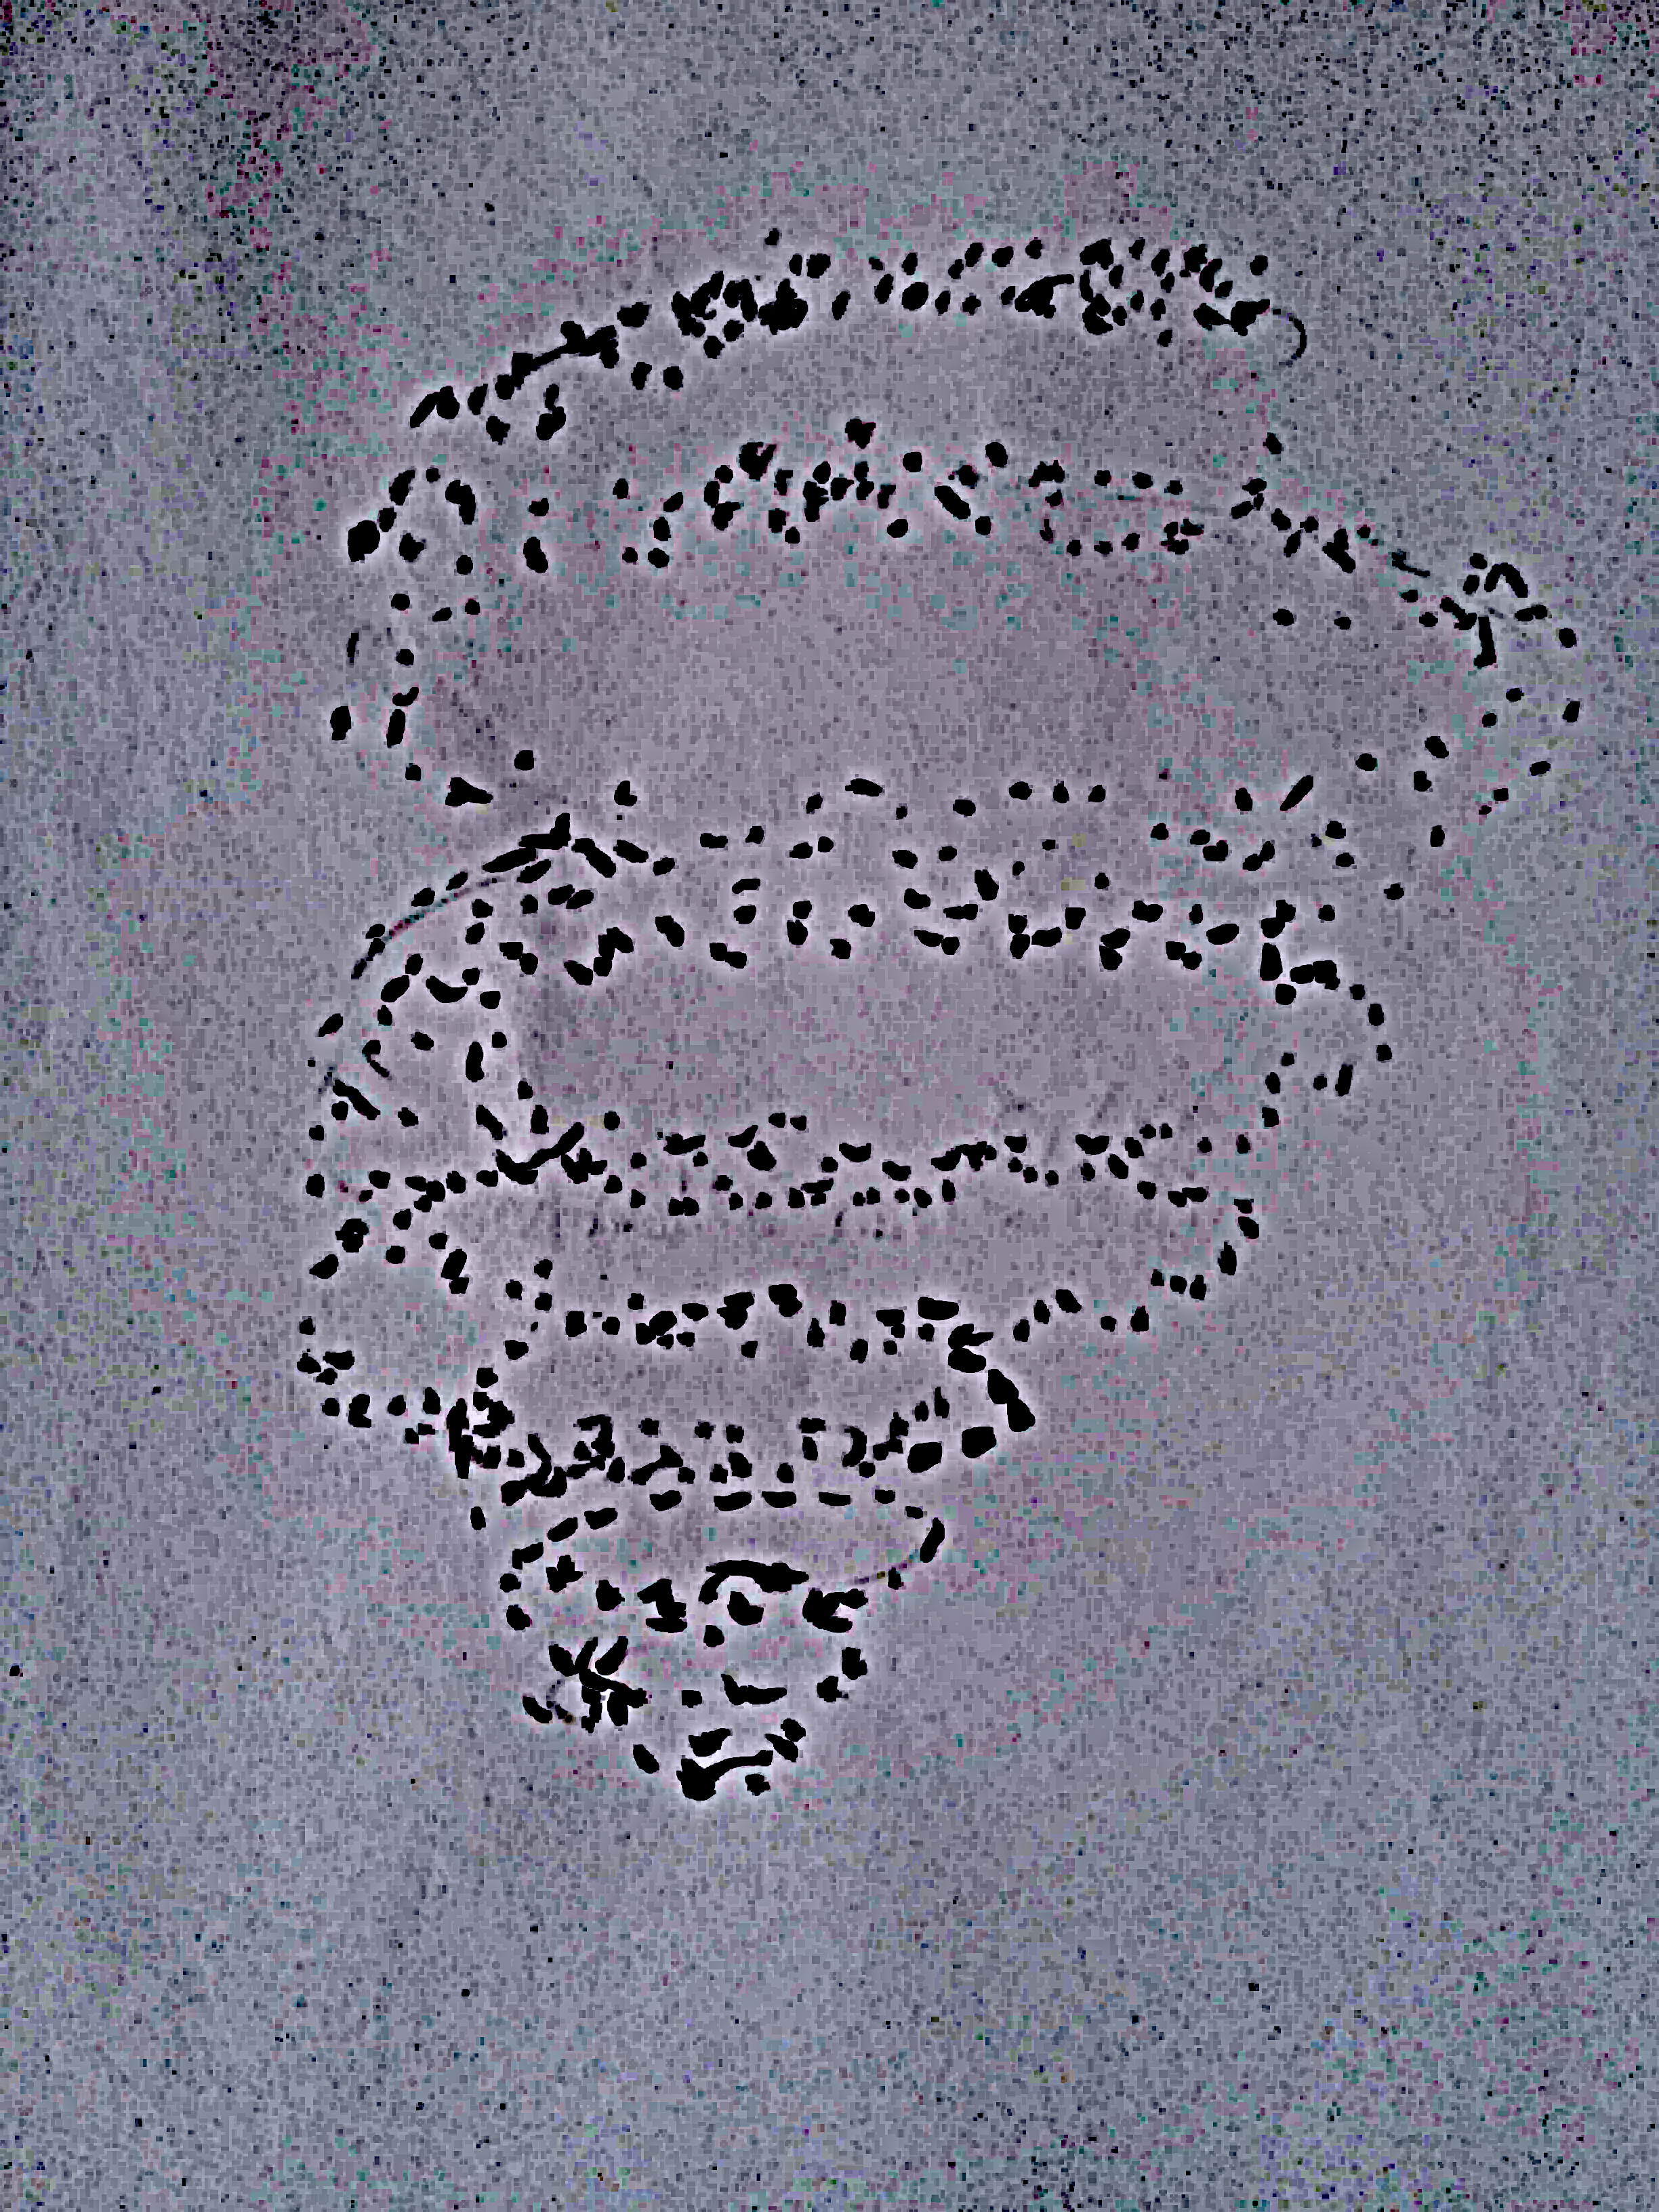
\includegraphics[width=.5\paperwidth,height=\paperheight,angle=0]{nube_moscas}};
	\node [inner sep=0pt, minimum width=.55\paperwidth, minimum height=\paperheight,opacity=1,xshift=-.2\paperwidth,text width=.55\linewidth] at (current page.center) {Y SI PRIMERO ERAN 2 MOSCAS, UN SEGUNDO DESPUÉS ERAN 4, LUEGO DE OTRO SEGUNDO, 8$\ldots$ ¿CUÁNTAS SERÍAN EN 30 SEGUNDOS?
		
		SI UNA MOSCA PESA APROXIMADAMENTE 20 MILIGRAMOS (¡ES DECIR, 0.020 GRAMOS!), ¿CUANTO PESARÍA TODA ESA CANTIDAD DE MOSCAS? ÉSTAS Y OTRAS PREGUNTAS ME HACÍA MIENTRAS UNA NUBE INFERNAL IBA CRECIENDO DESCONTROLADAMENTE.};		
	
	
\end{tikzpicture}

\newpage
\begin{tikzpicture}[remember picture, overlay]
	\node [inner sep=0pt, minimum width=\paperwidth, minimum height=\paperheight,opacity=.5] at (current page.center) {\includegraphics[width=\paperwidth,height=\paperheight,angle=0]{paper21}};
	\node[text width=.85\paperwidth,xshift=0\paperwidth,yshift=0cm,scale=1] at (current page.center){
		ERA UN REMOLINO FENOMENAL, EL ZUMBIDO HABÍA CRECIDO A NIVELES INSOPORTABLES, ¡TENÍA QUE ESCAPAR DE ALLÍ!
		
		ESCUCHÉ LOS MAULLIDOS DE AKIS QUE ME LLAMABA, SEGURAMENTE TRATANDO ÉL MISMO DE LUCHAR CONTRA LA TRAMPA MORTAL QUE NOS HABÍAN JUGADO.
		
		YO YA NO VEÍA NADA Y SENTÍA QUE MI CABEZA DABA VUELTAS INTERMINABLES, COMO SI EL REMOLINO ME HUBIESE LEVANTADO COMO UN TORNADO. LOS COLORES SE DILUÍAN Y TODO SE VOLVÍA MÁS OSCURO. ESO NO ESTÁ TAN MAL PARA UN GATO NEGRO, QUE SABE QUE TIENE VENTAJAS SI NO HAY LUZ, PERO ADMITO QUE ME ASUSTÉ BASTANTE PORQUE NO SENTÍA BIEN MIS PATAS, ¡PARECÍA ESTAR DENTRO DE UN SUEÑO!
	};
\end{tikzpicture}

\newpage
\begin{tikzpicture}[remember picture, overlay]
	\node [inner sep=0pt, minimum width=\paperwidth, minimum height=\paperheight,opacity=.8] at (current page.center) {\includegraphics[width=\paperwidth,height=\paperheight,angle=0]{paper20}};
	\node [inner sep=0pt, minimum width=\paperwidth, minimum height=.5\paperheight,opacity=1,xshift=0\paperwidth,yshift=.3\textheight] at (current page.center) {\includegraphics[height=.5\paperheight,angle=0]{reina_mosca}};
	\node [inner sep=0pt, minimum width=.9\paperwidth, minimum height=\paperheight,opacity=1,xshift=0\paperwidth,text width=.95\linewidth,yshift=-.2\paperheight] at (current page.center) {DESPERTÉ Y VI UNA IMAGEN HORRENDA, ¡NO PODÍA CREER LO QUE LLEGABA A MIS PUPILAS!. UNA MOSCA DE PROPORCIONES IRREALES SE HALLABA FRENTE A MÍ, REVOLOTEANDO SOBRE SU LUGAR, MIRÁNDOME CON SUS MÚLTIPLES Y ESPANTOSOS OJOS. PARECÍA PODER LEER SU MENTE, ME DIJO:
		
		-¡INSENSATO! PENSASTE QUE PODRÍAS SALIRTE CON LA TUYA, PEQUEÑO DEPREDADOR!};		
	
\end{tikzpicture}

\newpage
\begin{tikzpicture}[remember picture, overlay]
	\node [inner sep=0pt, minimum width=\paperwidth, minimum height=\paperheight,opacity=.8] at (current page.center) {\includegraphics[width=\paperwidth,height=\paperheight,angle=0]{paper20}};
	
\end{tikzpicture}
MI PRIMERA REACCIÓN FUE INTENTAR CORRER, PERO NO ERA CLARO HACIA DONDE PODÍA HUIR Y ESA ESPECIE DE REINA MOSCA GIGANTE TENÍA UNA PRESENCIA HIPNÓTICA. 

MAULLÉ PERO NO ESCUCHABA CLARAMENTE. LA MOSCA SEGUÍA LEYENDO MI MENTE Y AGREGÓ:

-JAJA, ESTÁS EN UN SUEÑO DE MOSCAS, MI AMIGO FELINO.

JAMÁS SERÉ AMIGO DE ESTOS HORRIPILANTES BICHOS, PENSÉ. 

-SOY UNA MOSCA MUY ESPECIAL, VENGO DE MUY LEJOS. DE UN LUGAR QUE DE SEGURO NO TE IMAGINAS. Y CON TU PATÉTICO AMIGO PENSARON QUE PODÍAN ACABARNOS CON FACILIDAD, PERO YA VES$\ldots$

-¿DONDE ESTÁ MI AMIGO?, PROTESTÉ. 

-PRONTO PODRÁN REUNIRSE, POR AHORA, NO PODRÁS ESCAPAR DE AQUÍ.




\newpage
\begin{tikzpicture}[remember picture, overlay]
	\node [inner sep=0pt, minimum width=\paperwidth, minimum height=\paperheight,opacity=.8] at (current page.center) {\includegraphics[width=\paperwidth,height=\paperheight,angle=0]{paper20}};
	
\end{tikzpicture}
-¿DONDE ESTOY?

- ¡EN UN LUGAR DONDE NADIE PODRÁ ENCONTRARTE!

LO DIJO CON UNA VOZ TENEBROSA, COMO LAS DE ESAS PELÍCULAS QUE DAN MIEDO A LOS HUMANOS. A MÍ MUCHO NO ME ASUSTAN PORQUE SUELEN SER PERSONAJES LENTOS Y TROPES, INCAPACES DE ALCANZAR A UN INTRÉPIDO FELINO COMO YO.

-ESO LO VEREMOS, MAULLÉ Y CORRÍ HACIA LA DIRECCIÓN OPUESTA DE DONDE ESTABA LA MOSCA. A LOS POCOS METROS ENCONTRÉ UNA PARED RUGOSA Y HÚMEDA. COMENCÉ A SEGUIR LA PARED, CON VELOCIDAD. PERO ME DÍ CUENTA PRONTO DE QUE DABA VUELTAS COMO EN CÍRCULO.

LA MOSCA HABÍA DESAPARECIDO Y SE DISIPÓ UN TANTO LA OSCURIDAD. ME DI CUENTA DE QUE ME HALLABA DENTRO DE UN PEQUEÑO PATIO INTERNO, RODEADO DE ALTAS PAREDES. PARECÍA DIFÍCIL DE TREPAR, PERO IGUAL LO INTENTÉ.

\newpage
\begin{tikzpicture}[remember picture, overlay]
	\node [inner sep=0pt, minimum width=\paperwidth, minimum height=\paperheight,opacity=.8] at (current page.center) {\includegraphics[width=\paperwidth,height=\paperheight,angle=0]{paper20}};
	
	
\end{tikzpicture}
PERO NO DESESPERÉ. LOS GATOS TENEMOS MUCHA PACIENCIA. ME PUSE A DORMITAR Y PENSAR EN ALGUNA FORMA DE ESCALAR LAS PAREDES, DE APROVECHAR CADA IMPERFECCIÓN QUE PUDIERA AYUDARME A TREPAR CON MIS GARRITAS. 

ME ANIMABA SABER QUE PODÍA MOVERME YA BIEN Y QUE EL SUEÑO NO ME DOMINABA, AÚN SI LOS RAYOS DE SOL QUE LLEGABAN ERA CADA VEZ MÁS POCOS. LOS GATOS TENEMOS MUY BUENAS PUPILAS EN ESTOS CASOS. 

TREPÉ DE UN SALTO DE UNA PARED A OTRA Y ME ENCONTRABA COMO A 2 METROS DEL SUELO, ¿ERA UN AVANCE! PERO MIS PATAS CEDIERON Y TUVE QUE DEJARME CAER CON ESTILO.

VOLVÍA A PREPARARME, SIN TEMOR, CUANDO ESCUCHÉ UNA VOZ FAMILIAR:

-¡OTTOKO! ¿DONDE ESTÁS MI FELINITO?




\newpage
\begin{tikzpicture}[remember picture, overlay]
	\node [inner sep=0pt, minimum width=\paperwidth, minimum height=\paperheight,opacity=.8] at (current page.center) {\includegraphics[width=\paperwidth,height=\paperheight,angle=0]{paper6}};
\end{tikzpicture}	
-¿MIAU?	, RESPONDÍ.

-¡OTTOKO!, ¡SOS VOS! DIJO LA MISMA VOZ CON ALEGRÍA. MIRÉ HACIA ARRIBA Y POR ENCIMA DE LA PARED DISTINGUÍ LA FIGURA DE MI CUIDADOR, DE MI PADRE HUMANO. Y FUE UN ALIVIO, IBA A PODER SALIR DEL LUGAR DONDE ME ENCONTRABA

VI CAER UNA SOGA MUY GRUESA, MUCHO MÁS ANCHA DE ESAS QUE SUELO MORDER EN CASA. POR SUPUESTO QUE LE DI UN BUEN ZARPAZO Y HASTA UNA POTENTE MORDIDA Y ENTENDÍ QUE DEBÍA AFERRARME A ELLA PARA PODER ESCALAR BIEN ALTO.

-¡MUY BIEN, OTTOKO, BRAVO, SEGUÍ ASÍ!

ALENTADO, ESCALÉ SIN PROBLEMAS LA SOGA HASTA LLEGAR A SUS BRAZOS.

ALLÍ ARRIBA  VI A AKIS. COMPRENDÍ QUE PROBABLEMENTE HUBIESE IDO POR AYUDA. 




\newpage
\begin{tikzpicture}[remember picture, overlay]
	\node [inner sep=0pt, minimum width=\paperwidth, minimum height=\paperheight,opacity=1] at (current page.center) {\includegraphics[width=\paperwidth,height=\paperheight,angle=0]{alivio}};
\end{tikzpicture}	
A VECES, INCLUSO LOS MÁS PODEROSOS GATOS NECESITAMOS UNA MANO AMIGA PARA VENCER DIFICULTADES.

MI PADRE ME PUSO ENSEGUIDA DENTRO DE UNA MOCHILA, COMO  HACE CUANDO ME LLEVA A LA VETERINARIA. 

-¡OTTOKO! ¡ESTABA MUY PREOCUPADO!,

DIJO ENTRE ENOJADO Y ALIVIADO. 

ME ACARICIABA LA CABEZA REVOLVIENDO

MI PROLIJOS PELOS.

VOLVIMOS A CASA Y ALLÍ, DESPUÉS DE 

TOMAR MUCHA AGUA Y COMER MIS 

CROQUETAS, DORMÍ COMO CUANDO ERA 

PEQUEÑITO.


\newpage
\begin{tikzpicture}[remember picture, overlay]
	\node [inner sep=0pt, minimum width=\paperwidth, minimum height=\paperheight,opacity=.8] at (current page.center) {\includegraphics[width=\paperwidth,height=\paperheight,angle=0]{paper6}};
\end{tikzpicture}

¡HABÍA SIDO UNA TODA UNA HISTORIA! ¿EXISTIRÍA EN ALGÚN LUGAR ESA HORRIBLE MOSCA GIGANTE? 

AL DÍA SIGUIENTE ENTENDÍ TODO LO QUE HABÍA OCURRIDO. CON AKIS HABÍAMOS ATACADO A LA NUBE DE MOSCAS Y FUE UN ATMÓSFERA ALGO VENENOSA QUE LLEGÓ A CONFUNDIR MIS SENTIDOS.
EXISTEN EN EL ÁFRICA UNA CLASE DE MOSCAS QUE SON LLAMADAS MOSCAS TSE TSE, O LAS MOSCAS QUE PROVOCAN EL SUEÑO. PUEDEN AFECTAR A LOS MAMÍFEROS EN GENERAL Y CREO QUE ME PROVOCARON ESAS DESAGRADABLES ALUCINACIONES.

DEBO HABER ESTADO ALGO ASÍ COMO SONÁMBULO, ME DIJO AKIS, PUES EL VIÓ QUE YO ME PERDÍ SOLO, TREPANDO EN LA CASA Y BAJANDO A SU PATIO. MI AMIGO NO PUDO RESCATARME Y FUE EN BUSCA DE AYUDA. 


\newpage
\begin{tikzpicture}[remember picture, overlay]
	\node [inner sep=0pt, minimum width=\paperwidth, minimum height=\paperheight,opacity=.8] at (current page.center) {\includegraphics[width=\paperwidth,height=\paperheight,angle=0]{paper20}};
\end{tikzpicture}
MAULLÓ AL LADO DE NUESTRO HOGAR Y MI PADRE LO SIGUIÓ HASTA DAR CON LA CASA ABANDONADA. COMPRÓ CORREAS EN UNA FERRETERÍA Y PIDIÓ ACCESO A UN VECINO PARA ALCANZAR LA TERRAZA Y ASÍ DARME UNA SALIDA DEL PATIO.

POR SUERTE TODO TERMINÓ BIEN, UN FINAL TRANQUILO Y FELIZ. POR LAS DUDAS NO VOLVIMOS A AVENTURARNOS CERCA DE ESA CASA MISTERIOSA, PUES NECESITA SEGURAMENTE VENTILACIÓN PARA SANEARSE.
